% Options for packages loaded elsewhere
\PassOptionsToPackage{unicode}{hyperref}
\PassOptionsToPackage{hyphens}{url}
%
\documentclass[
]{book}
\usepackage{amsmath,amssymb}
\usepackage{iftex}
\ifPDFTeX
  \usepackage[T1]{fontenc}
  \usepackage[utf8]{inputenc}
  \usepackage{textcomp} % provide euro and other symbols
\else % if luatex or xetex
  \usepackage{unicode-math} % this also loads fontspec
  \defaultfontfeatures{Scale=MatchLowercase}
  \defaultfontfeatures[\rmfamily]{Ligatures=TeX,Scale=1}
\fi
\usepackage{lmodern}
\ifPDFTeX\else
  % xetex/luatex font selection
\fi
% Use upquote if available, for straight quotes in verbatim environments
\IfFileExists{upquote.sty}{\usepackage{upquote}}{}
\IfFileExists{microtype.sty}{% use microtype if available
  \usepackage[]{microtype}
  \UseMicrotypeSet[protrusion]{basicmath} % disable protrusion for tt fonts
}{}
\makeatletter
\@ifundefined{KOMAClassName}{% if non-KOMA class
  \IfFileExists{parskip.sty}{%
    \usepackage{parskip}
  }{% else
    \setlength{\parindent}{0pt}
    \setlength{\parskip}{6pt plus 2pt minus 1pt}}
}{% if KOMA class
  \KOMAoptions{parskip=half}}
\makeatother
\usepackage{xcolor}
\usepackage{color}
\usepackage{fancyvrb}
\newcommand{\VerbBar}{|}
\newcommand{\VERB}{\Verb[commandchars=\\\{\}]}
\DefineVerbatimEnvironment{Highlighting}{Verbatim}{commandchars=\\\{\}}
% Add ',fontsize=\small' for more characters per line
\usepackage{framed}
\definecolor{shadecolor}{RGB}{248,248,248}
\newenvironment{Shaded}{\begin{snugshade}}{\end{snugshade}}
\newcommand{\AlertTok}[1]{\textcolor[rgb]{0.94,0.16,0.16}{#1}}
\newcommand{\AnnotationTok}[1]{\textcolor[rgb]{0.56,0.35,0.01}{\textbf{\textit{#1}}}}
\newcommand{\AttributeTok}[1]{\textcolor[rgb]{0.13,0.29,0.53}{#1}}
\newcommand{\BaseNTok}[1]{\textcolor[rgb]{0.00,0.00,0.81}{#1}}
\newcommand{\BuiltInTok}[1]{#1}
\newcommand{\CharTok}[1]{\textcolor[rgb]{0.31,0.60,0.02}{#1}}
\newcommand{\CommentTok}[1]{\textcolor[rgb]{0.56,0.35,0.01}{\textit{#1}}}
\newcommand{\CommentVarTok}[1]{\textcolor[rgb]{0.56,0.35,0.01}{\textbf{\textit{#1}}}}
\newcommand{\ConstantTok}[1]{\textcolor[rgb]{0.56,0.35,0.01}{#1}}
\newcommand{\ControlFlowTok}[1]{\textcolor[rgb]{0.13,0.29,0.53}{\textbf{#1}}}
\newcommand{\DataTypeTok}[1]{\textcolor[rgb]{0.13,0.29,0.53}{#1}}
\newcommand{\DecValTok}[1]{\textcolor[rgb]{0.00,0.00,0.81}{#1}}
\newcommand{\DocumentationTok}[1]{\textcolor[rgb]{0.56,0.35,0.01}{\textbf{\textit{#1}}}}
\newcommand{\ErrorTok}[1]{\textcolor[rgb]{0.64,0.00,0.00}{\textbf{#1}}}
\newcommand{\ExtensionTok}[1]{#1}
\newcommand{\FloatTok}[1]{\textcolor[rgb]{0.00,0.00,0.81}{#1}}
\newcommand{\FunctionTok}[1]{\textcolor[rgb]{0.13,0.29,0.53}{\textbf{#1}}}
\newcommand{\ImportTok}[1]{#1}
\newcommand{\InformationTok}[1]{\textcolor[rgb]{0.56,0.35,0.01}{\textbf{\textit{#1}}}}
\newcommand{\KeywordTok}[1]{\textcolor[rgb]{0.13,0.29,0.53}{\textbf{#1}}}
\newcommand{\NormalTok}[1]{#1}
\newcommand{\OperatorTok}[1]{\textcolor[rgb]{0.81,0.36,0.00}{\textbf{#1}}}
\newcommand{\OtherTok}[1]{\textcolor[rgb]{0.56,0.35,0.01}{#1}}
\newcommand{\PreprocessorTok}[1]{\textcolor[rgb]{0.56,0.35,0.01}{\textit{#1}}}
\newcommand{\RegionMarkerTok}[1]{#1}
\newcommand{\SpecialCharTok}[1]{\textcolor[rgb]{0.81,0.36,0.00}{\textbf{#1}}}
\newcommand{\SpecialStringTok}[1]{\textcolor[rgb]{0.31,0.60,0.02}{#1}}
\newcommand{\StringTok}[1]{\textcolor[rgb]{0.31,0.60,0.02}{#1}}
\newcommand{\VariableTok}[1]{\textcolor[rgb]{0.00,0.00,0.00}{#1}}
\newcommand{\VerbatimStringTok}[1]{\textcolor[rgb]{0.31,0.60,0.02}{#1}}
\newcommand{\WarningTok}[1]{\textcolor[rgb]{0.56,0.35,0.01}{\textbf{\textit{#1}}}}
\usepackage{longtable,booktabs,array}
\usepackage{calc} % for calculating minipage widths
% Correct order of tables after \paragraph or \subparagraph
\usepackage{etoolbox}
\makeatletter
\patchcmd\longtable{\par}{\if@noskipsec\mbox{}\fi\par}{}{}
\makeatother
% Allow footnotes in longtable head/foot
\IfFileExists{footnotehyper.sty}{\usepackage{footnotehyper}}{\usepackage{footnote}}
\makesavenoteenv{longtable}
\usepackage{graphicx}
\makeatletter
\def\maxwidth{\ifdim\Gin@nat@width>\linewidth\linewidth\else\Gin@nat@width\fi}
\def\maxheight{\ifdim\Gin@nat@height>\textheight\textheight\else\Gin@nat@height\fi}
\makeatother
% Scale images if necessary, so that they will not overflow the page
% margins by default, and it is still possible to overwrite the defaults
% using explicit options in \includegraphics[width, height, ...]{}
\setkeys{Gin}{width=\maxwidth,height=\maxheight,keepaspectratio}
% Set default figure placement to htbp
\makeatletter
\def\fps@figure{htbp}
\makeatother
\setlength{\emergencystretch}{3em} % prevent overfull lines
\providecommand{\tightlist}{%
  \setlength{\itemsep}{0pt}\setlength{\parskip}{0pt}}
\setcounter{secnumdepth}{5}
\usepackage{booktabs}  
\usepackage{float}     
\let\cleardoublepage\clearpage  

% Fix table of contents blank pages
\usepackage{etoolbox}
\makeatletter
\patchcmd{\tableofcontents}{\cleardoublepage}{\clearpage}{}{}
\makeatother

% Ensure headings do not appear alone at the bottom of a page
\usepackage{titlesec}
\usepackage{needspace}
\usepackage{lmodern}  

% Keep section headings with at least 5 lines of content
\let\oldsection\section
\renewcommand{\section}{\needspace{5\baselineskip}\oldsection}

\let\oldsubsection\subsection
\renewcommand{\subsection}{\needspace{3\baselineskip}\oldsubsection}  % Move only if less than 3 lines fit

\let\oldsubsubsection\subsubsection
\renewcommand{\subsubsection}{\needspace{2\baselineskip}\oldsubsubsection}  % Smallest headings need 2 lines

% Prevents 'titlesec' errors if the package is missing
\ifdefined\titleformat
  % titlesec is loaded
\else
  \usepackage{titlesec}
\fi

\usepackage{fancyhdr}
\pagestyle{plain}  % Removes headers, keeps page numbers at the bottom
\ifLuaTeX
  \usepackage{selnolig}  % disable illegal ligatures
\fi
\usepackage[]{natbib}
\bibliographystyle{apalike}
\usepackage{bookmark}
\IfFileExists{xurl.sty}{\usepackage{xurl}}{} % add URL line breaks if available
\urlstyle{same}
\hypersetup{
  pdftitle={StartR for Psychology at Royal Holloway},
  pdfauthor={Luke Kendrick},
  hidelinks,
  pdfcreator={LaTeX via pandoc}}

\title{StartR for Psychology at Royal Holloway}
\author{Luke Kendrick}
\date{2025-04-09}

\begin{document}
\maketitle

{
\setcounter{tocdepth}{1}
\tableofcontents
}
\chapter{Welcome to StartR}\label{welcome-to-startr}

StartR is a short course for someone who wants a beginner's guide to using R and RStudio. This resource is suitable for anyone who wants a gentle self-paced introduction.

\begin{figure}

{\centering 
\includegraphics[width=0.25\linewidth]{images/pirate_spaced} 

}

\caption{**R** is not just the sound a pirate makes, but it is also a programming language.}\label{fig:fig1}
\end{figure}

\section{What is R and RStudio?}\label{what-is-r-and-rstudio}

R is a programming language for statistical computing and data visualisation (see \url{https://www.r-project.org/about.html}). As with any language, you could write a set of instructions or operations for someone to follow.

For example, I could ask you to:

\begin{Shaded}
\begin{Highlighting}[]
\StringTok{\textasciigrave{}}\AttributeTok{stand up}\StringTok{\textasciigrave{}}\NormalTok{ and then,}
\StringTok{\textasciigrave{}}\AttributeTok{walk towards the window}\StringTok{\textasciigrave{}}\NormalTok{ and then,}
\StringTok{\textasciigrave{}}\AttributeTok{return to your seat}\StringTok{\textasciigrave{}}
\end{Highlighting}
\end{Shaded}

I hope you enjoyed looking out of the window for a moment there. We will come back to this later, but the basic logic behind code is writing a series of instructions.

When using R, you'll be giving instructions to our computer to follow and complete.

R is not the same thing as RStudio. RStudio is an integrated development environment (IDE). It provides a user-friendly interface for you to add your instructions and to view output.

Think of the difference between R and RStudio in the same way you would a car dashboard and an engine. The engine of the car works in the background and unless you're a mechanic, it will just work away in the background without much notice. Being seated in the car with the dashboard on the other hand is where you direct or drive your car. RStudio is how you will drive whilst R (the coding language under the hood) is the engine underneath. This book will show you how to drive and to understand how the engine works, but it is really not necessary to become a mechanic, just a good driver!

\section{Installing R and RStudio}\label{installing-r-and-rstudio}

With installation you will need both the car dashboard \textbf{and} the engine. You should install two things:

\begin{itemize}
\tightlist
\item
  R (the engine)
\item
  RStudio (the car dashboard)
\end{itemize}

You can install both of these here.

\section{Opening RStudio}\label{opening-rstudio}

Once you have installed both of these, you should only open \textbf{RStudio}.

Find RStudio on your computer and open it. The RStudio logo is shown in Figure \ref{fig:fig2}. A frequent mistake is opening the engine \texttt{R}, but you should only use RStudio.

\begin{figure}

{\centering 
\includegraphics[width=0.25\linewidth]{images/RStudio} 

}

\caption{Look out for the RStudio logo.}\label{fig:fig2}
\end{figure}

When you open RStudio it should look like the screenshot in Figure \ref{fig:fig3}. Notice that there are three main panels.

\begin{figure}

{\centering 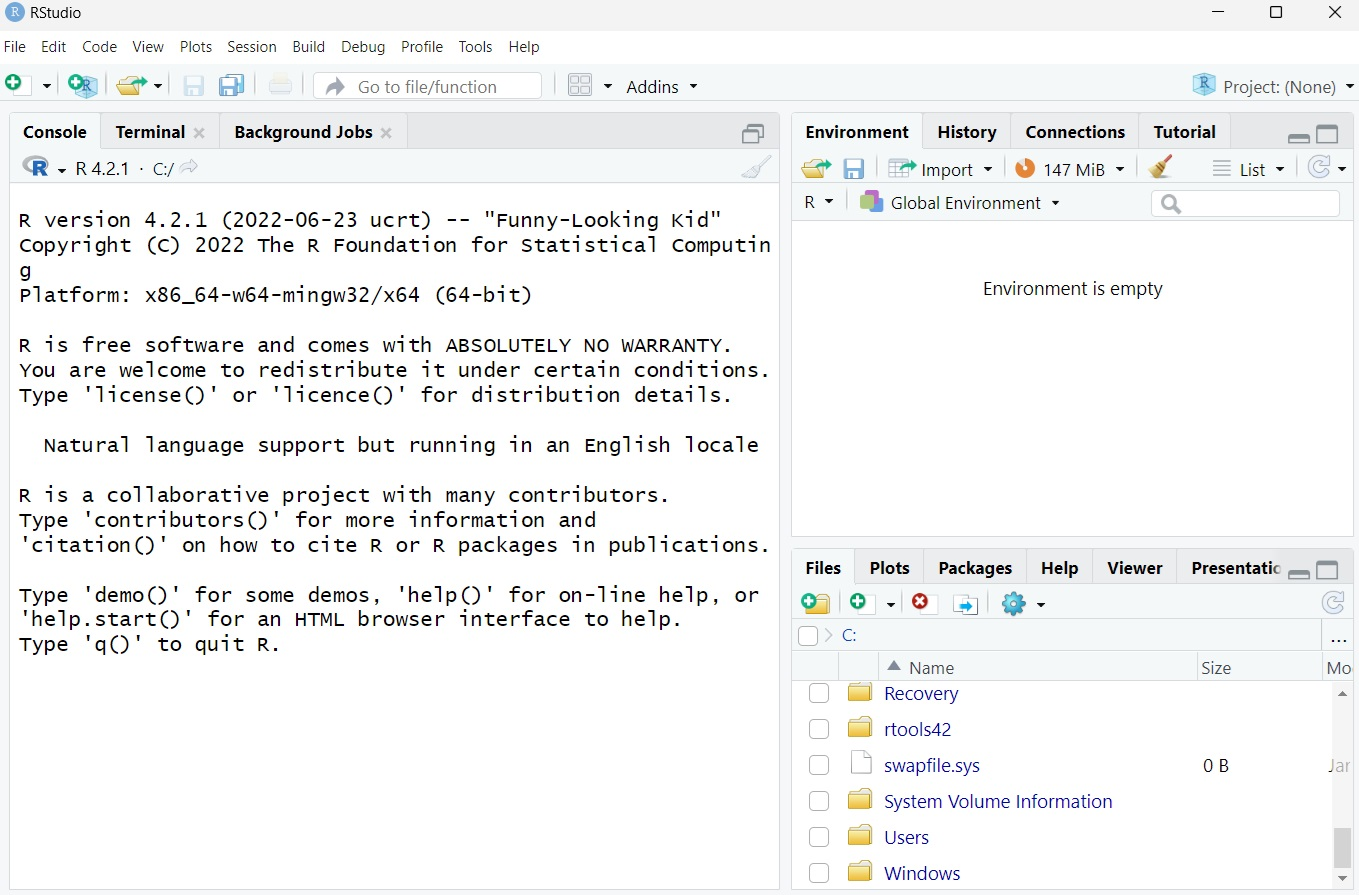
\includegraphics[width=1\linewidth]{images/rstudio1} 

}

\caption{RStudio when first opened.}\label{fig:fig3}
\end{figure}

Before you really dive in to getting RStudio to work, you will need to open a new script. To do this, look for the top left button which looks like a blank white page with a green/white \texttt{plus} symbol, just like in Figure \ref{fig:fig4} below.

\begin{figure}

{\centering 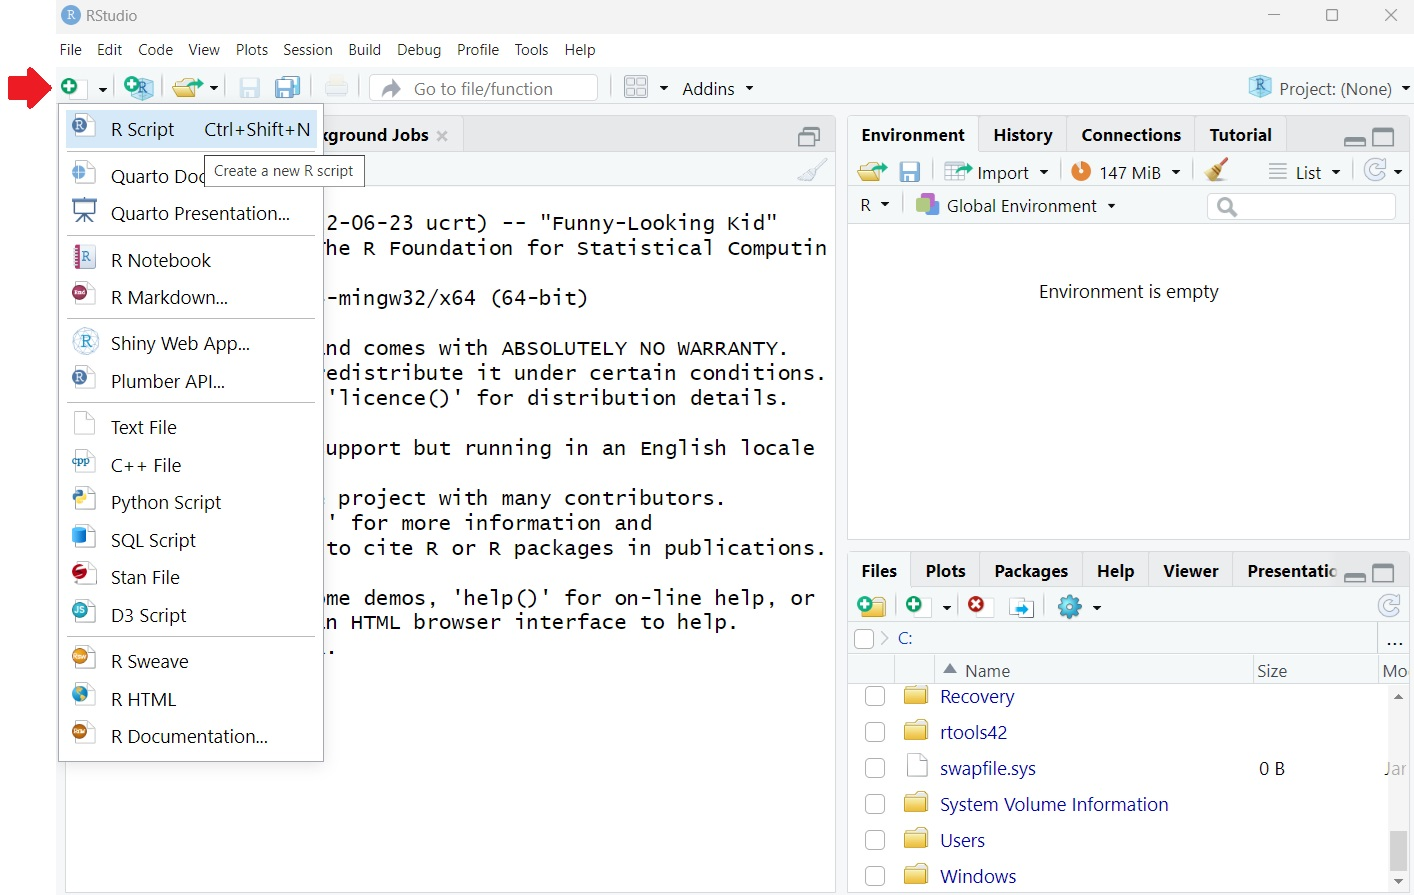
\includegraphics[width=1\linewidth]{images/rscript} 

}

\caption{Open a new R Script.}\label{fig:fig4}
\end{figure}

Once you open the new script you should now see four panels just like Figure \ref{fig:fig5}.

\begin{figure}

{\centering 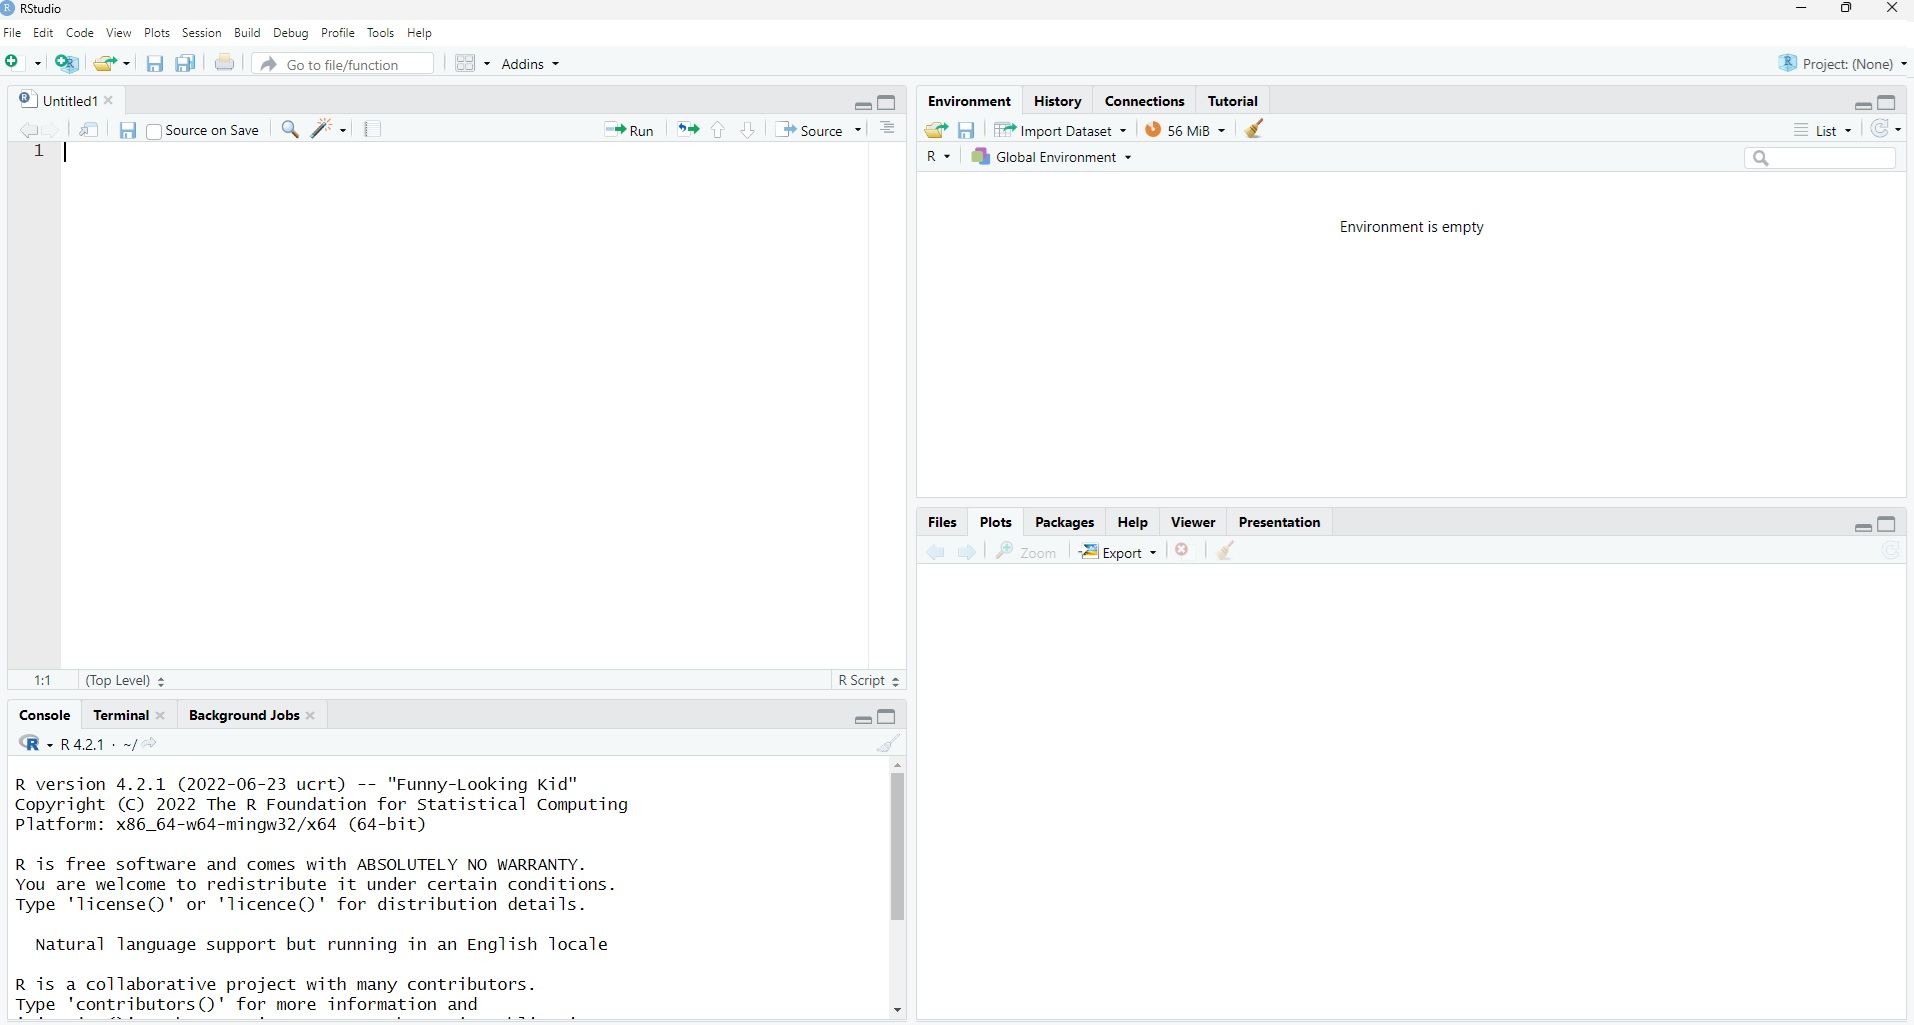
\includegraphics[width=1\linewidth]{images/rstudio2} 

}

\caption{You should see four panels now which means you are ready to start working with RStudio.}\label{fig:fig5}
\end{figure}

Another way to open a new script is to use the menu at the top of the RStudio window: \texttt{File\ \textgreater{}\ New\ File\ \textgreater{}\ R\ Script}.

\section{A Quick Tour of RStudio}\label{a-quick-tour-of-rstudio}

Now it is time to learn about the four panels. Let's go through each one by one. These four panels are shown in Figure \ref{fig:fig6} with a description of each below.

\begin{figure}[H]

{\centering 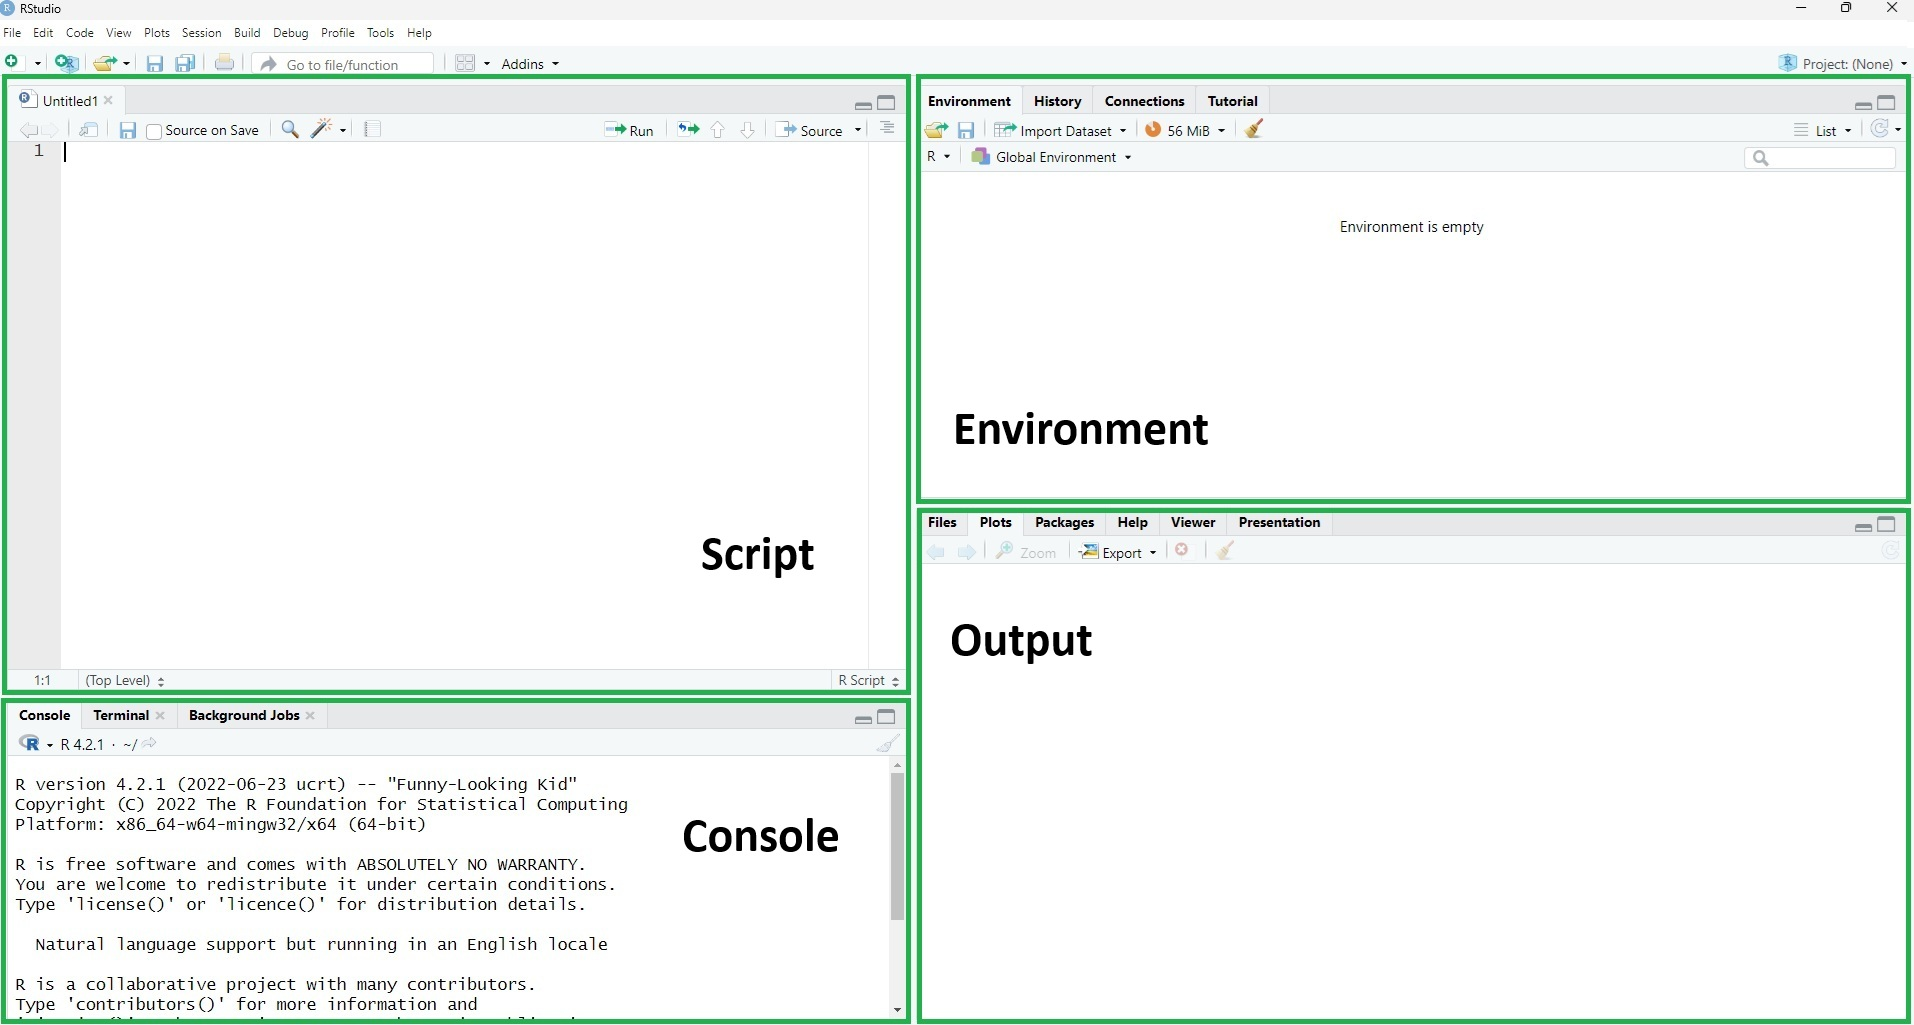
\includegraphics[width=1\linewidth]{images/rstudio3} 

}

\caption{The four panels in RStudio.}\label{fig:fig6}
\end{figure}

\textbf{Script Panel}

This is the top left panel. This is an editable space where you will be able to type and edit any code you use. The good news is you can save an R script so you can use it again in the future.

Think of it as an input panel.

\textbf{Console Panel}

The bottom left panel is the console. Whilst you can technically type in any code here, I'd advise you not to as you wont be able to save any code. The console is where you can view any output messages. Essentially, once you type in and run your code in the script, RStudio will respond to you via this console panel.

Think of it as an output panel.

\textbf{Environment Panel}

This is the top right panel. This is a space where RStudio will hold any \texttt{objects}. Essentially this is a bit like a memory space where RStudio will keep hold of any important information you ask it to.

Think of it as a memory panel.

\textbf{Output Panel}

The bottom right panel is a bit trickier to name. I will call it the output panel but ultimately it can do a few jobs. You might notice different tabs. \texttt{Plots} is where we will see any data visualisation outputs, or plots. \texttt{Packages} provides a list of our packages (more on this later). \texttt{Help} is also a useful tab as it is a space where you read about R Documentation (instructions how to use bits of code). There is also a \texttt{files} tab which can allow you to navigate files on your computer.

\section{Chapter Summary}\label{chapter-summary}

At the end of this chapter you should have installed R and RStudio. You should have also opened RStudio and created a new script so that you can see four panels.

Take a few moments to have a little look around these four panels so that you are familiar with what they look like before the next chapter.

\chapter{Putting R to Work}\label{putting-r-to-work}

In this chapter you will start using code and putting RStudio to work! We will begin with very basic code so that you become familiar with the layout and how entering code works.

\section{What Day is it Today?}\label{what-day-is-it-today}

Let's begin with something really simple.

When RStudio is open you want to make sure you have four panels, with the top left panel (script) open and ready. This is where you can type your code.

Type the code below into your script now.

\begin{Shaded}
\begin{Highlighting}[]
\FunctionTok{date}\NormalTok{()}
\end{Highlighting}
\end{Shaded}

Once you have typed in your code, you are ready to run it. This means you will ask RStudio to tell you today's date.

To run the code you can leave your cursor at the end of the line of code and use your keyboard to press \texttt{Control} + \texttt{Enter} or \texttt{Command} + \texttt{Enter} on a Mac. You might also notice on the top right of your script panel there is a button called \texttt{run}. This will also run the line of code but I'd recommend getting used to using the keyboard.

\newpage

Once you have run the line of code, take a look at the \textbf{console} (bottom left panel). If it has worked you should see today's date:

\begin{Shaded}
\begin{Highlighting}[]
\FunctionTok{date}\NormalTok{()}
\CommentTok{\#\textgreater{} [1] "Wed Apr  9 13:31:00 2025"}
\end{Highlighting}
\end{Shaded}

Congratulations! You have entered the world of coding.

Well, what else can RStudio do? It can be helpful to also think of the script panel as a very fancy calculator. With this in mind, let's try out some maths sums. Run the following code:

\begin{Shaded}
\begin{Highlighting}[]
\DecValTok{20}\SpecialCharTok{+}\DecValTok{80}
\end{Highlighting}
\end{Shaded}

If you ran it successfully you should see the answer appear in the \textbf{console} (bottom left panel).

Next, try a really complex sum:

\begin{Shaded}
\begin{Highlighting}[]
\DecValTok{12345}\SpecialCharTok{*}\DecValTok{54321}
\end{Highlighting}
\end{Shaded}

Note that we need to use \texttt{*} an asterisk to signify this is a multiplication sum. Run the line of code and check out the answer. In case you needed to know the answer to 12345 x 54321, RStudio is there for you!

Hopefully now you are starting to see the very basics of how you should input code into RStudio and where to check to see the output.

\section{Functions and Arguments: A Piece of Pi}\label{functions-and-arguments-a-piece-of-pi}

In the previous section, you ran a bit of code which is a \textbf{function} called \texttt{date()}. In R, a \textbf{function} is a bit of code that performs a specific task. Functions have parentheses \texttt{()} at the end, for example \texttt{date()} is a function which returns the current date and time.

An \textbf{argument} is a piece of information that you pass into a function, which will change the way the function behaves. Let's look at an example.

The code below will use the function called \texttt{round()}. Within this function (inside the parentheses) I can enter an \textbf{argument}. I've entered the mathematical constant pi here as the argument.

The function \texttt{round()} with pi \texttt{π} entered as an argument (inside the parentheses) will just round the value to the nearest whole number. Try this yourself in RStudio now.

\begin{Shaded}
\begin{Highlighting}[]
\FunctionTok{round}\NormalTok{(}\FloatTok{3.14159265359}\NormalTok{)}
\CommentTok{\#\textgreater{} [1] 3}
\FunctionTok{round}\NormalTok{(pi) }\CommentTok{\# or you can just type \textasciigrave{}pi\textasciigrave{}}
\CommentTok{\#\textgreater{} [1] 3}
\end{Highlighting}
\end{Shaded}

However, what if I wanted this output to two-decimal places? No problem! Simply add another argument. Some functions will contain multiple arguments, but for now let's keep it simple.

Run the code below and check your console to see the output.

\begin{Shaded}
\begin{Highlighting}[]
\FunctionTok{round}\NormalTok{(}\FloatTok{3.14159265359}\NormalTok{, }\AttributeTok{digits =} \DecValTok{2}\NormalTok{)}
\end{Highlighting}
\end{Shaded}

Here we have use a \texttt{,} comma to separate the arguments within the parentheses. The argument \texttt{digits\ =\ 2} can be used to change the behaviour of this function by rounding pi \texttt{π} to two decimal places. An \textbf{argument} will give a function some more specific guidance.

As you advance further with R code you'll be using lots of different functions and arguments.

If at any point you want to learn about a function, we can use \texttt{?}. Try running the code below:

\begin{Shaded}
\begin{Highlighting}[]
\NormalTok{?}\FunctionTok{round}\NormalTok{()}
\end{Highlighting}
\end{Shaded}

If you ran it successfully you will notice in the \textbf{output panel} (bottom right) that the \textbf{help} tab is now showing documentation to explain how this function works, including all the possible arguments.

You can use \texttt{?} at any time to see how a function works.

\section{Comments = Human Notes}\label{comments-human-notes}

You might be a little worried that eventually you are going to have to remember so much code. The base version of R contains thousands of functions, even before we start using \textbf{packages}! (more on packages later). One concern people have with code is needing to remember everything.

To deal with this issue, when writing our code, we should use comments in our R script. A \textbf{comment} is a piece of text which you can add next to your code as a note. I like to think of comments as ``human notes'', we can read them but RStudio will ignore them.

In order to tell RStudio where our human notes begin we need to use \texttt{\#} hashtag. Anything written after the hashtag is not processed or read by RStudio. Check out the example below:

\begin{Shaded}
\begin{Highlighting}[]
\FunctionTok{date}\NormalTok{() }\CommentTok{\#this will ask for today\textquotesingle{}s date}

\FunctionTok{round}\NormalTok{(}\FloatTok{3.14159265359}\NormalTok{, }\AttributeTok{digits =} \DecValTok{2}\NormalTok{) }\CommentTok{\#this rounds a value to two decimal places}
\end{Highlighting}
\end{Shaded}

Rstudio will run those \textbf{functions} but the notes are there for your benefit. You should use notes routinely when writing code for two important reasons:

\begin{enumerate}
\def\labelenumi{\arabic{enumi}.}
\item
  It will help remind you how your code works if you look at it again in the future.
\item
  If you send or share your code with someone else, your notes can help them to understand what you've done and why.
\end{enumerate}

Therefore, here we have our first important rule:

\begin{quote}
\textbf{Always make use of comments when coding in RStudio (\#)}
\end{quote}

Before moving on to the next section, head back into RStudio and practice adding some notes to your R script. Remember to use the \texttt{\#} hashtag. Once you've finished writing your notes, hit enter and then the script moves to the next line ready for the next bit of code.

\section{Creating Objects}\label{creating-objects}

Another important feature is knowing how to create an \textbf{object}. Variables and/or data can be assigned to objects, however, you need to create the object yourself. Let's look at an example. Run the code below:

\begin{Shaded}
\begin{Highlighting}[]
\NormalTok{myobject }\OtherTok{\textless{}{-}} \FunctionTok{c}\NormalTok{(}\DecValTok{1}\NormalTok{, }\DecValTok{2}\NormalTok{, }\DecValTok{3}\NormalTok{, }\DecValTok{4}\NormalTok{)}
\end{Highlighting}
\end{Shaded}

Let's talk through this code step by step:

\begin{itemize}
\item
  What you might notice is that I have created an object called \texttt{myobject} (a truly inspirational name). This is on the very left of this line of code. You can call an object anything you like, so feel free to call it something else.
\item
  Next I have used an arrow \texttt{\textless{}-}. This means that anything written on the right hand side of this arrow will be committed to this object. This arrow is called an assignment operator.
\item
  Then I used \texttt{c()} which is a function that allows us to list values. I created a mini data set with the numbers 1-4.
\end{itemize}

Go ahead if you haven't already and run that bit of code, nothing particularly thrilling will happen and you may notice that the console does not return anything exciting. However, take a look at the \textbf{environment} panel (top right) and what do you notice?

If it has worked, you should spot that there is an object called \texttt{myobject} (or whatever you called yours) as shown in Figure \ref{fig:fig-environment}.

\begin{figure}[H]

{\centering 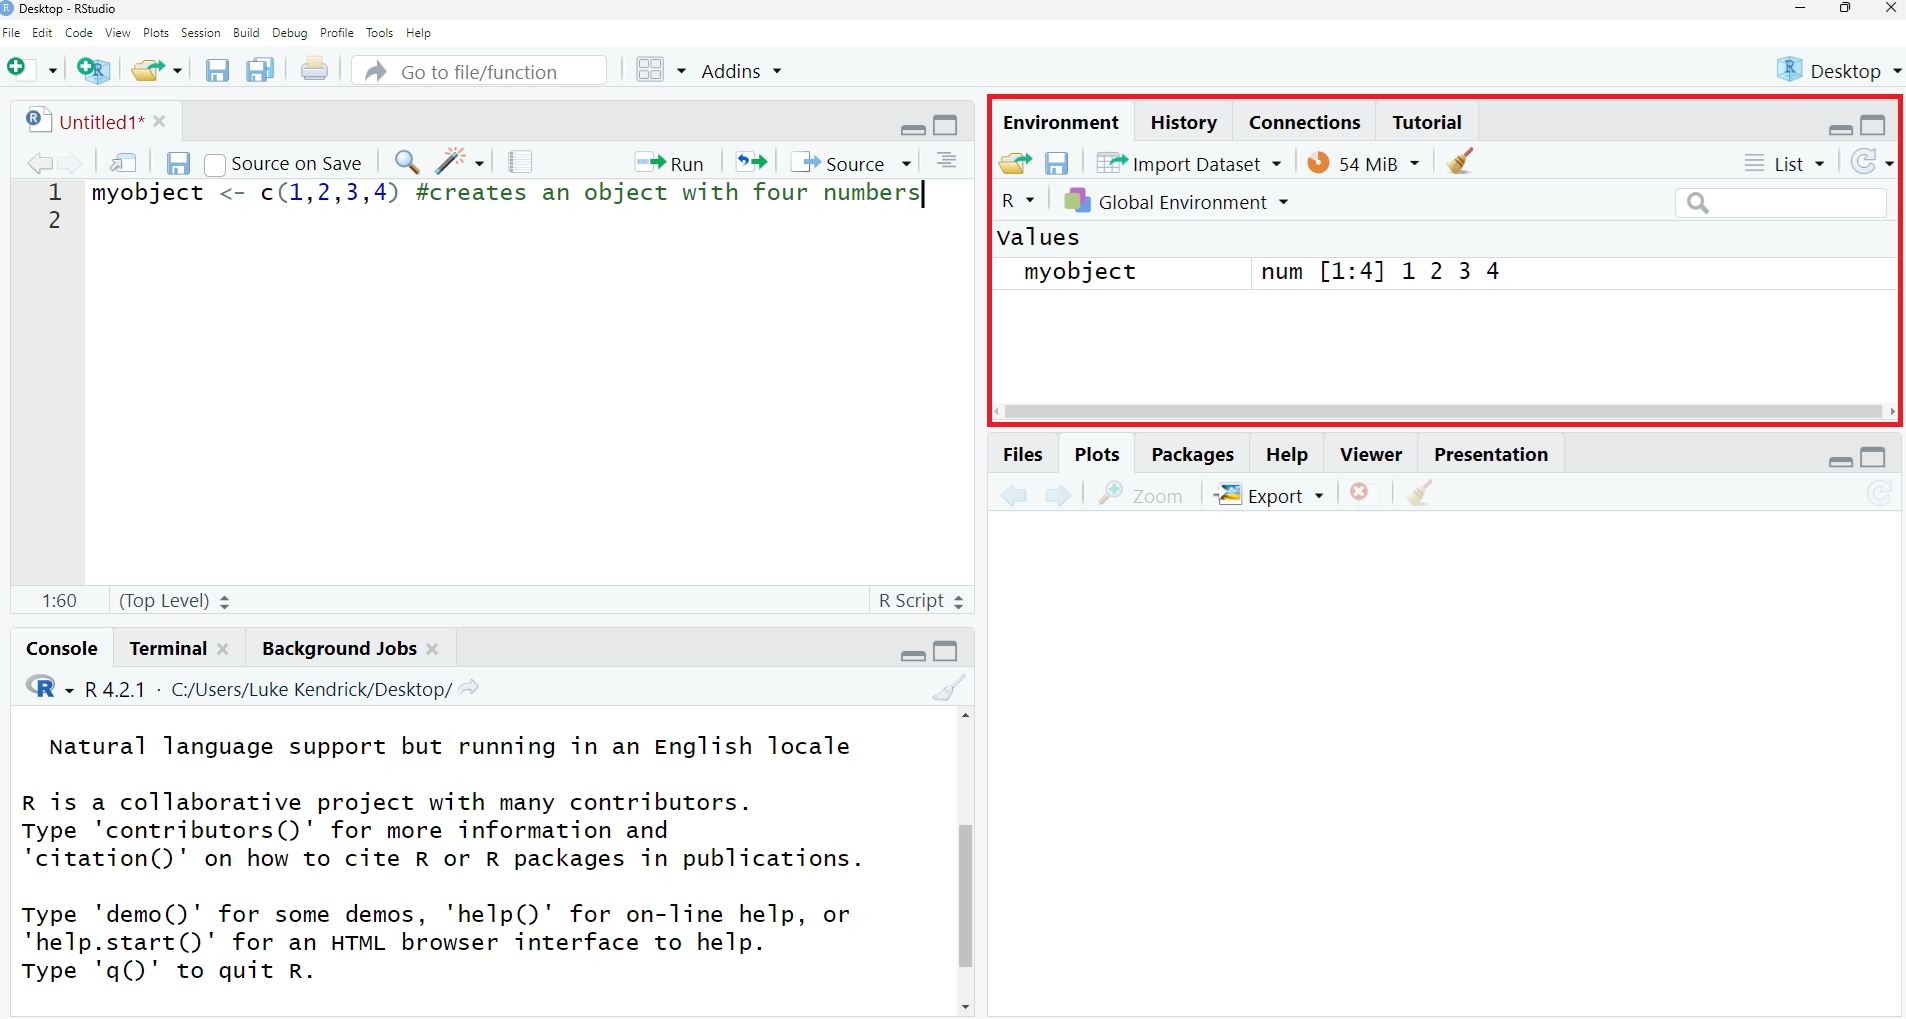
\includegraphics[width=1\linewidth]{images/object} 

}

\caption{The environment contains the new object called `myobject`.}\label{fig:fig-environment}
\end{figure}

\begin{quote}
In the R world:

\begin{itemize}
\item
  Everything that exists is an object.
\item
  Everything that happens is a function.
\end{itemize}
\end{quote}

Almost anything can be committed to an object in RStudio. For example, run and adapt the code below. Change ``Luke'' to your own name! Then check that your environment looks like Figure \ref{fig:fig-environment-1}.

\begin{Shaded}
\begin{Highlighting}[]
\NormalTok{name }\OtherTok{\textless{}{-}} \StringTok{"Luke"}
\NormalTok{answer }\OtherTok{\textless{}{-}} \DecValTok{12345}\SpecialCharTok{*}\DecValTok{54321}
\NormalTok{pi }\OtherTok{\textless{}{-}} \FunctionTok{round}\NormalTok{(}\FloatTok{3.14159265359}\NormalTok{, }\AttributeTok{digits =} \DecValTok{2}\NormalTok{)}
\end{Highlighting}
\end{Shaded}

\begin{figure}[H]

{\centering 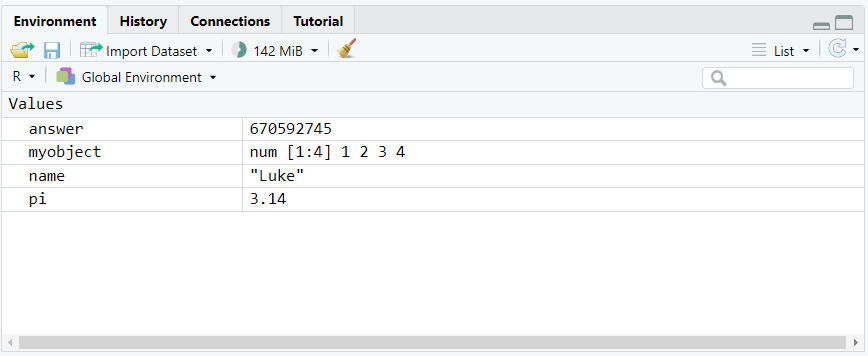
\includegraphics[width=1\linewidth]{images/environment} 

}

\caption{The environment contains multiple new objects.}\label{fig:fig-environment-1}
\end{figure}

We can also print an object to the console. Essentially this will ask RStudio to just show the contents of an object in the console. You should try this with the \texttt{print()} function, see below.

\begin{Shaded}
\begin{Highlighting}[]
\FunctionTok{print}\NormalTok{(myobject)}
\FunctionTok{print}\NormalTok{(name)}
\FunctionTok{print}\NormalTok{(answer)}
\FunctionTok{print}\NormalTok{(pi)}
\end{Highlighting}
\end{Shaded}

\subsection{\texorpdfstring{\textbf{Naming and Removing Objects}}{Naming and Removing Objects}}\label{naming-and-removing-objects}

I did say that you can call an object anything you like. One thing that will help is to try and keep object names short. That is because often you might need to keep typing out object names, particularly if you use the object frequently (e.g., an object that contains your data set for analysis).

Generally, avoid using multiple words and keep it short and informative.

\begin{Shaded}
\begin{Highlighting}[]
\NormalTok{what\_is\_my\_first\_name }\OtherTok{\textless{}{-}} \StringTok{"Luke"} \CommentTok{\# this is not a good object name. it is too long.}
\NormalTok{name }\OtherTok{\textless{}{-}} \StringTok{"Luke"} \CommentTok{\# this is a short informative object name}
\end{Highlighting}
\end{Shaded}

Finally, if you want to remove an object from your environment you can use the code below:

\begin{Shaded}
\begin{Highlighting}[]
\FunctionTok{rm}\NormalTok{(myobject, name, answer, pi) }\CommentTok{\# will remove these four objects.}

\FunctionTok{rm}\NormalTok{(}\AttributeTok{list =} \FunctionTok{ls}\NormalTok{()) }\CommentTok{\# will remove EVERYTHING from the environment.}
\end{Highlighting}
\end{Shaded}

\section{Troubleshooting and Getting Help with R}\label{troubleshooting-and-getting-help-with-r}

During the early stages of learning to code it is not uncommon to come across error messages. Sometimes the code will not work and this can be frustrating. Also, some error messages are a little tricky to interpret. Thankfully there are options for support to troubleshoot issues.

Firstly, remember to use \texttt{?} in front of a function to check out the documentation to ensure you are using it correctly. If I wanted to learn about the \texttt{rm()} function from the previous section I would use:

\begin{Shaded}
\begin{Highlighting}[]
\NormalTok{?}\FunctionTok{rm}\NormalTok{()}
\end{Highlighting}
\end{Shaded}

Secondly, if you come across an error message and you cannot figure it out/it looks a load of gibberish, copy and paste the error message into Google. It is likely that someone else would have experienced this error and there is probably a solution already online.

Finally, one of the most common issues when learning to code is the presence of a typo. When you code in RStudio it needs to be written very specifically and how it expects it to be written. RStudio will not work if you make a typo. Similarly, R code is case sensitive. \texttt{myobject} is not the same as \texttt{MYOBJECT} or \texttt{mYobject}.

Take your time to check you code carefully when you are starting out in R, most errors tend to be small typos.

Therefore, here we have our second important rule:

\begin{quote}
\textbf{Check your code for typos and enter it exactly as R expects}
\end{quote}

\section{Chapter Summary}\label{chapter-summary-1}

You should now have an understanding of how functions and arguments work. You should also have ran your very first lines of code! Congratulations, you are officially an R coder. You should also now be able to create objects, name them appropriately, and remove them from the environment. Finally, you should be aware of two key rules: (1) use comments to make notes with you code and (2) enter code exactly intended and check out for typos. In the next chapter you will begin to work with packages and learn how to import a data set into RStudio ready for data analysis.

\chapter{Packages and Importing Data}\label{packages-and-importing-data}

In this chapter we will cover two important features of RStudio. Firstly is the use of packages. Packages allow you to access a variety of different functions. Additionally, before you begin working with any data you will need to somehow actually get that data into RStudio via a working directory.

\section{What are Packages?}\label{what-are-packages}

When you first open RStudio, you will have access to many base R functions. In fact there are a great deal of functions that exist in the base version of R. In fact, you have already used some in the previous chapter, for example, \texttt{date()} or \texttt{round()} are considered base R functions.

Base R is essentially the ``basic subscription'' version of RStudio without any additional apps installed.

Often we might need some quite specialised functions. In order to access these we need to install and load \texttt{packages}. You can think of \texttt{packages} as a bit like your mobile phone apps\ldots in that you need to download them, install them, and then open them to access their specific functions.

One \textbf{key} package that is required for learning and using R for Psychology at Royal Holloway is the \texttt{tidyverse} package. \texttt{Tidyverse} is essentially a collection of packages, see more \href{https://www.tidyverse.org/}{here}.

\subsection{Installing a Package}\label{installing-a-package}

Tidyverse is already installed on most Royal Holloway campus computers and so this step is not necessary. But still worth a read as in future you may need to install other packages beyond the tidyverse.

To install tidyverse we can use the \texttt{install.packages()} function. See below:

\begin{Shaded}
\begin{Highlighting}[]
\FunctionTok{install.packages}\NormalTok{(}\StringTok{"tidyverse"}\NormalTok{) }\CommentTok{\# install the tidyverse package}
\end{Highlighting}
\end{Shaded}

Note you'll see I also followed my own advice and used human notes with the hashtag \texttt{\#}.

You'll notice that the name of the package needs to be in quotation marks. When you run this line of code, RStudio will get to work installing the package. It might take a couple of minutes and you will see this happening in the console (bottom left panel).

\subsection{Loading a Package}\label{loading-a-package}

Just because you have installed a package does not yet mean you are ready to use it. Next you need to load it. To do this you can use the \texttt{library()} function below:

\begin{Shaded}
\begin{Highlighting}[]
\FunctionTok{library}\NormalTok{(tidyverse) }\CommentTok{\# load the tidyverse package}
\end{Highlighting}
\end{Shaded}

Note that we do not need to use quote marks.

Remember, you only need to install a package once on your computer. However, each time you reopen RStudio (whether at home or on a campus PC), you'll need to load the necessary libraries using the \texttt{library()} function.

\subsection{Checking Packages}\label{checking-packages}

You can check which packages you have installed and loaded at anytime. Head to the ``packages'' tab on the bottom right panel. If the package is listed then it is installed. If there is a tick in the box on the left, that also means the package has been loaded and is ready to go! Why not try and un-tick and then tick tidyverse in this panel and see what happens in the console. See Figure \ref{fig:fig-environment-3} below.

\begin{figure}[H]

{\centering 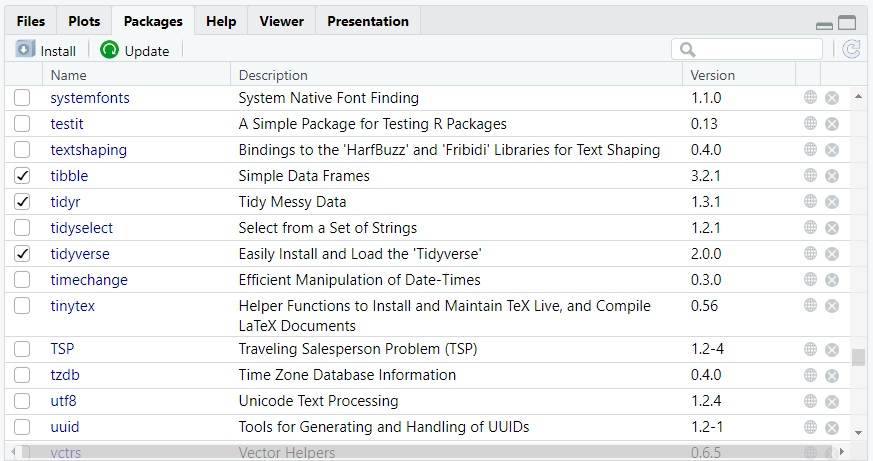
\includegraphics[width=0.95\linewidth]{images/packages} 

}

\caption{An example of the packages tab with the Tidyverse package loaded.}\label{fig:fig-environment-3}
\end{figure}

\section{Importing Data}\label{importing-data}

Now we have Tidyverse loaded, you can begin thinking about importing some data. There are different way to import data, and you might actually notice an \texttt{Import\ Dataset} in the environment panel. However, the best way to import data is via a \texttt{Working\ Directory} and using a Tidyverse function called \texttt{read\_csv}. Let's go through this bit by bit.

\subsection{Set the Working Directory}\label{set-the-working-directory}

The working directory is a folder on your computer that RStudio will look in to find any data files. It is also where RStudio can save any output files too.

Before setting your working directory it is important to think about your file structure on your computer. For example, you might consider creating a special folder to save any of your RStudio work. You can then link this special folder to RStudio using the steps below.

Head to the \texttt{Session} tab at the top of the RStudio window and then select \texttt{Set\ Working\ Directory} -\textgreater{} \texttt{Choose\ Directory}. See Figure \ref{fig:fig-environment-4} below.

\begin{figure}[H]

{\centering 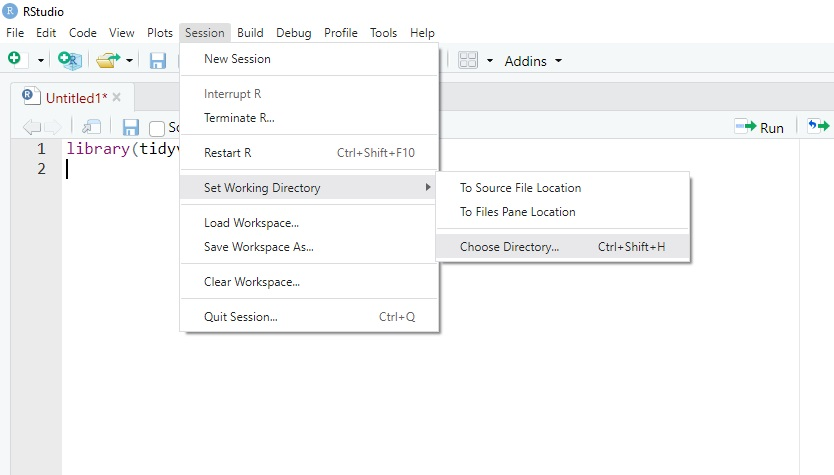
\includegraphics[width=0.8\linewidth]{images/setwd} 

}

\caption{Set the working directory}\label{fig:fig-environment-4}
\end{figure}

This will open up a file browser on your computer. Select the folder on your computer that you have designated as your \texttt{Working\ Directory}. The one in Figure \ref{fig:fig-environment-5} is called \texttt{R\_Folder} but you might call yours something else if you like, for example, \texttt{StartR}. You'll notice that the folder I have selected below is empty because it is a new folder with nothing in it\ldots yet!

\begin{figure}[H]

{\centering 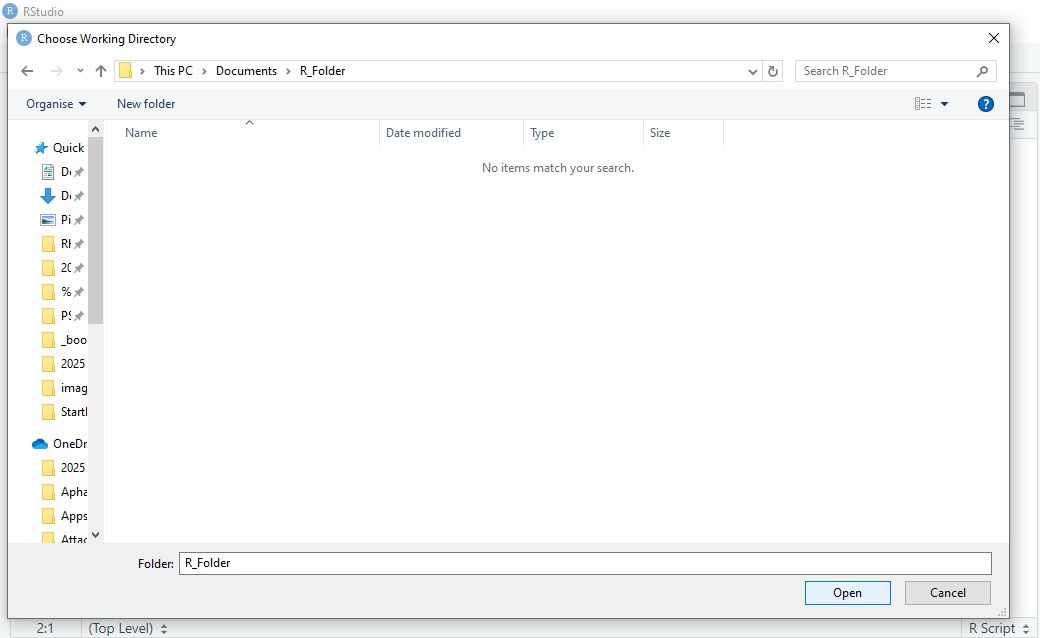
\includegraphics[width=0.75\linewidth]{images/setwd2} 

}

\caption{Head into the folder that you will use as your working directory in this session}\label{fig:fig-environment-5}
\end{figure}

In case you forget, you can check your working directory at any point using this line of code:

\begin{Shaded}
\begin{Highlighting}[]
\FunctionTok{getwd}\NormalTok{() }\CommentTok{\# will check the current working directory.}
\end{Highlighting}
\end{Shaded}

You should see in the console (bottom left) that RStudio will tell you the location of the folder on your computer that is now your designated working directory.

\subsection{Importing Data}\label{importing-data-1}

RStudio primarily likes to work with a file format called \texttt{.csv}. This stands for comma separated values. There are ways to import other types of files (e.g., SPSS, excel, text) but during this course we will only work with \texttt{.csv} files.

Let's try and get a basic data set in to RStudio. Download the data set below and \emph{remember} save it into your designated working directory folder. For reference, the data are also presented below.

\href{data/height.csv}{Download the data set}

\begin{longtable}[]{@{}lll@{}}
\caption{A table of ten people containing their age (in years) and height (in cm).}\tabularnewline
\toprule\noalign{}
id & age & height \\
\midrule\noalign{}
\endfirsthead
\toprule\noalign{}
id & age & height \\
\midrule\noalign{}
\endhead
\bottomrule\noalign{}
\endlastfoot
1 & 22 & 167 \\
2 & 26 & 178 \\
3 & 18 & 173 \\
4 & 32 & 169 \\
5 & 19 & 183 \\
6 & 39 & 172 \\
7 & 41 & 159 \\
8 & 46 & 164 \\
9 & 32 & 153 \\
10 & 25 & 159 \\
\end{longtable}

\subsection{read\_csv()}\label{read_csv}

Once the data file is in your working directory folder we can try to import it using \texttt{read\_csv()}.

\begin{Shaded}
\begin{Highlighting}[]
\NormalTok{data }\OtherTok{\textless{}{-}} \FunctionTok{read\_csv}\NormalTok{(}\StringTok{"height.csv"}\NormalTok{) }\CommentTok{\# import the height.csv data set and save it as an object called \textasciigrave{}data\textasciigrave{}.}
\end{Highlighting}
\end{Shaded}

This line of code here begins to combine everything we have covered in this StartR short course so far. Take a moment ro work through the explanations below to ensure you understand:

\begin{itemize}
\item
  \texttt{data} is an \textbf{object}. I have called it data as it is just a short 4 letter word and is our data set.
\item
  \texttt{\textless{}-} is the \textbf{assignment operator}. It will assign things to the right side to our object on the left side called \texttt{data.}
\item
  \texttt{read\_csv()} is a \textbf{function} which will read data from a .csv file.
\item
  \texttt{"height.csv"} is an \textbf{argument} which tells the function how to behave. In this case it will look for a specific file called height.csv.
\item
  It will look for this file in the \texttt{working\ directory}.
\item
  If this works successfully you should see an object called \texttt{data} in the \textbf{environment} panel (top right), see Figure \ref{fig:fig-environment-6}.
\item
  Notice that ``height.csv'' is spelled exactly to match the file name. No capital letters or spaces, which is how it appeared when you downloaded it.
\end{itemize}

\begin{figure}[H]

{\centering 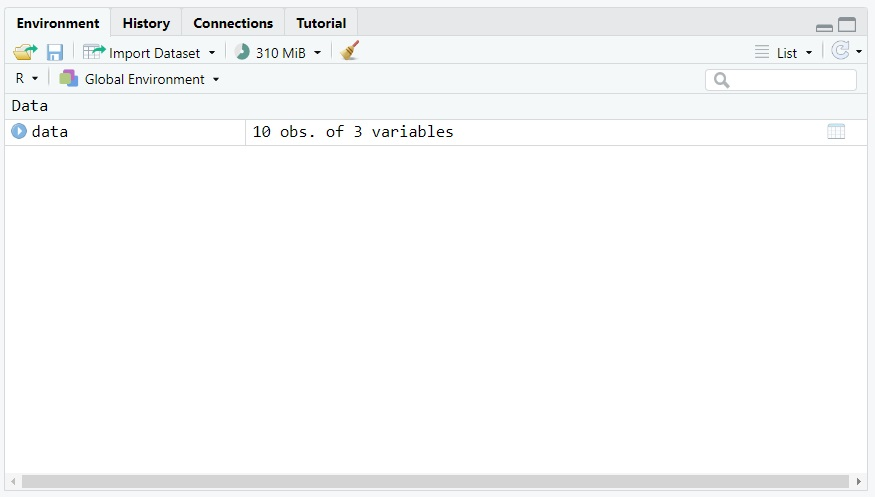
\includegraphics[width=0.75\linewidth]{images/importdata} 

}

\caption{The environment panel with the newly created `data` object}\label{fig:fig-environment-6}
\end{figure}

You might also notice there is some very basic information visible to the right of the object in the environment. For example, there are \texttt{10\ obs.\ of\ 3\ variables}. This tells us there are 10 observations across three different variables.

Finally, if you double click on the object name \texttt{data}, it will open the data file in a new tab.

You can also achieve the same result using:

\begin{Shaded}
\begin{Highlighting}[]
\FunctionTok{view}\NormalTok{(data) }\CommentTok{\# will open the data in a new tab}
\end{Highlighting}
\end{Shaded}

A final note on \texttt{read\_csv()}.

You might learn that there is a similar function called \texttt{read.csv} (with a dot \texttt{.} not an underscore \texttt{\_}). Do not use read.csv. Always use the version with an underscore, which comes from the tidyverse package.

\subsection{Some (very) Basic Descriptive Statistics}\label{some-very-basic-descriptive-statistics}

In the final part of this chapter, you will calculate some very basic descriptive statistics. I wanted to minimise any ``stats'' stuff in this short course as the aim is really to learn about the RStudio layout and how it works before we properly work with data.

However, the code below will allow you to practice a little more understanding R functions, running code, and reading output.

We need a new package for this final section:

\begin{Shaded}
\begin{Highlighting}[]
\FunctionTok{install.packages}\NormalTok{(}\StringTok{"psych"}\NormalTok{) }\CommentTok{\# install Psych package}
\FunctionTok{library}\NormalTok{(psych) }\CommentTok{\# load the psych package}
\end{Highlighting}
\end{Shaded}

How about you work out some basic descriptive statistics for this data file. Using the \texttt{psych} package, you could use:

\begin{Shaded}
\begin{Highlighting}[]
\FunctionTok{describe}\NormalTok{(data) }\CommentTok{\# produce descriptive statistics}
\end{Highlighting}
\end{Shaded}

Run that now and check the output. The first line you might notice that id (identification number) has a mean of 5.50. This is meaningless and actually we could remove the ID column. How could we do this?

\subsection{Using the Pipe Operator}\label{using-the-pipe-operator}

Do you remember right at the start of chapter one I used the example below which is a three step command:

\begin{Shaded}
\begin{Highlighting}[]
\StringTok{\textasciigrave{}}\AttributeTok{stand up}\StringTok{\textasciigrave{}}\NormalTok{ and then,}
\StringTok{\textasciigrave{}}\AttributeTok{walk towards the window}\StringTok{\textasciigrave{}}\NormalTok{ and then,}
\StringTok{\textasciigrave{}}\AttributeTok{return to your seat}\StringTok{\textasciigrave{}}
\end{Highlighting}
\end{Shaded}

With our data we actually want to do the following which is also a three step command:

\begin{Shaded}
\begin{Highlighting}[]
\NormalTok{use }\StringTok{\textasciigrave{}}\AttributeTok{data}\StringTok{\textasciigrave{}}\NormalTok{ and then,}
\StringTok{\textasciigrave{}}\AttributeTok{remove id column}\StringTok{\textasciigrave{}}\NormalTok{ and then,}
\StringTok{\textasciigrave{}}\AttributeTok{describe}\StringTok{\textasciigrave{}}\NormalTok{ it.}
\end{Highlighting}
\end{Shaded}

We can use something called a pipe operator \texttt{\%\textgreater{}\%} which essentially means ``and then''. What will happen next is we will write out a set of instructions, line by line. Take a look at the code below and then run it:

\begin{Shaded}
\begin{Highlighting}[]
\NormalTok{data }\SpecialCharTok{\%\textgreater{}\%}
  \FunctionTok{select}\NormalTok{(}\SpecialCharTok{{-}}\NormalTok{id) }\SpecialCharTok{\%\textgreater{}\%}
  \FunctionTok{describe}\NormalTok{()}
\end{Highlighting}
\end{Shaded}

The three lines do the following:

\begin{enumerate}
\def\labelenumi{\arabic{enumi}.}
\item
  Take our object \texttt{data} \ldots and then\ldots{}
\item
  Use \texttt{select()} to remove id. We do this adding a minus sign \texttt{-} before id\ldots and then
\item
  \texttt{describe()} the results.
\end{enumerate}

Hopefully you can now see in the console the new output with the id column removed.

You will also see that the mean age was 30 years (SD = 9.64) and the mean height was 167.70 centimeters (SD = 9.25).

Congratulations! You have successfully produced some descriptive statistics.

\section{Chapter Summary}\label{chapter-summary-2}

In this chapter you have learnt about what packages can do for us. You might come across several different packages in the future and so you now know how to install packages and then load them. Another important task is being able to set the working directory. This is the folder on your computer that RStudio will use to find any data files. Next, you would have successfully imported a data file using read\_csv(). Finally, you should have use code to produce some very simple descriptive statistics.

  \bibliography{book.bib,packages.bib}

\end{document}
